\documentclass{article}
%\usepackage[a4paper, total={6in, 8in}]{geometry}
\usepackage{geometry}
 \geometry{
 a4paper,
 total={210mm,297mm},
 left=20mm,
 right=20mm,
 top=-2mm,
 bottom=2mm,
 }
%\usepackage[margin=0.5in]{geometry}

\usepackage{amsmath,amssymb}
\usepackage{ifpdf}
%\usepackage{cite}
\usepackage{algorithmic}
\usepackage{array}
\usepackage{mdwmath}
\usepackage{pdfpages}
\usepackage{mdwtab}
\usepackage{eqparbox}
\usepackage{cite}
%\onecolumn
%\input{psfig}
\usepackage{color}
\usepackage{graphicx}
\setlength{\textheight}{23.5cm} \setlength{\topmargin}{-1.05cm}
\setlength{\textwidth}{6.5in} \setlength{\oddsidemargin}{-0.5cm}
\renewcommand{\baselinestretch}{1}
\pagenumbering{arabic}
\usepackage{ragged2e}
\renewcommand{\baselinestretch}{1.5}

\begin{document}

\textbf{
\begin{center}
{
\large{School of Engineering and Applied Science (SEAS), Ahmedabad University}\vspace{4mm}
}
\end{center}
%
\begin{center}
\large{B.Tech(ICT) Semester IV: Probability and Random Processes (MAT 202) }\\ \vspace{3mm}
\end{center}
}
\begin{itemize}
\item Group No : S$\_$C3
\item Name (Roll No) : Prachee Javiya(AU1841032)\\\vspace{1mm}
\hspace{26mm} Panth Patel(AU1841020) \\\vspace{1mm}
\hspace{26mm} Dhruvil Dave(AU1841003)
\item Project Title: \textbf{The risk of a major nuclear accident: Calculation and perception of probabilities }

\end{itemize}

\section{Introduction}
\subsection{Background}
\begin{itemize}
    \item The whole of this paper is devoted to calculating the risk of a major nuclear accident.  By this we mean a failure initiating core meltdown. The cost of such accidents amounts to €1 per MWh generated. Setting aside the back of an envelope, which lends itself to quick, simple calculations, the paper gives us an insight into the accidents, from both a theoretical and an empirical standpoint. The study reports a probability of a core melt of $5\times10^{-5}$ per reactor year, in other words, a 0.00005 chance of an accident on a reactor operating for one year. Due to the confidentiality of data and limited resources, we would study one nuclear plant operating for 100,000 reactor years, rather than a fleet of 100000 reactors,operating for 1 year(The frequency remains unchanged)\cite{cite1}.The accident in Fukushima was caused by a tsunami (estimated to be 45 feet tall), which was due to the Tohoku earthquake on March 11; a pair of natural disasters that shut down the power and cooling of three nuclear reactors, leading to three nuclear meltdowns, and hydrogen air explosions. We will individually calculate the probabilities of above events and model them to analyse the risk of next possible nuclear accident.


    \item
    The main purpose of probabilistic safety assessments is not to estimate the probability of an accident on a specific plant or reactor, but rather to detect exactly what may go wrong, to identify the weakest links in the process and to understand the faults which most contribute to the risk of an accident. We will proceed methodically, starting from conditional probability, taking one branch of the tree and studying it deeper, calculating its probability and see how it affects the total probability. For example, Pr(release|melt|cooling system failure|loss of emergency power source|protective wall round plant breached by wave|7.0 magnitude quake)\cite{cite1}. All the possible sequences form an ‘event’ tree, with a series of forks, each branch being assigned a probability.

    \item Inside a nuclear reactor, slow thermal neutrons are bombarded inside the Uranium-235 core which react with the fuel and the Uranium present inside the fuel captures this slow moving electron and goes into an excited state and finally decays into residual, following a chain reaction. But what is the probability that this slow moving neutron reacts with the fuel? This is decided by a physical quantity which is called cross-section measured in barns(b). This quantity defines that with what amount of cross-section does this slow moving neutron reacts with and higher the cross-section, higher the probability of the reaction. This cross-section is measured w.r.t Incident Energy of slow moving neutron. After doing some mathematics and some quantum mechanical derivations, we get that cross-section formula turns out to be $\sigma = \pi \Bar{\lambda}^2 \frac{\Gamma^2}{(E - E_r)^2 + (\frac{\Gamma}{2})^2}$ which is known as a Breit-Wigner Distribution which is a modified form of Lorentz distribution. We can see that there is a peak in the distribution, which corresponds to $E_r$ which is called the Resonance Energy. At this peak we can see that cross-section is maximized which shows that if an incident Neutron is bombarded at this energy, it has a higher chance of reacting with the Nuclei.
\end{itemize}

\subsection{Motivation}
Nuclear Energy, by witnessing the gradual depletion of natural resources, "probably" will become the next primary source of energy in the near future.
Compared to other fuels, nuclear power costs relatively low (eradicating construction costs) and the likelihood of an accident occurring is also low, but when it does, it makes a huge dent in economic and environmental fabric ;a loss costing in billions(Fukushima Daiichi 11 Mar. 2011). The anomalies of the reaction are unpredictable and random which makes it difficult to track them.In today’s global energy environment, nuclear power plant managers need to consider many dimensions of risk in addition to nuclear safety-related risk.  In general we tend to overestimate any risk relating to rare, fearsome accidents. The purpose of this report is to provide an integrated framework for risk prediction as a tool to enhance the accuracy of predicting a major nuclear accident as well as risks associated with them, including core damage frequency. The reactions will be studied thoroughly in order to determine the output which contribute to a nuclear accident and what is the probability of an accident happening due to it . Things can go wrong in ways that we can not even foresee, we must collect data on all potential incidents that lead to the wrongdoing of a nuclear reactor thus creating a probabilistic model that provides a detailed risk analysis. Besides, who wouldn't want to get accurate answers to  universe's randomness?

\subsection{Problem statement}
This paper explores several probabilistic models and time series analysis methods for predicting the risk of a nuclear accident by determining the contribution of an event to a faulty   . The goal is to study individual events and predict the occurrence of a major nuclear accident in an area.
\begin{figure}
    \centering
  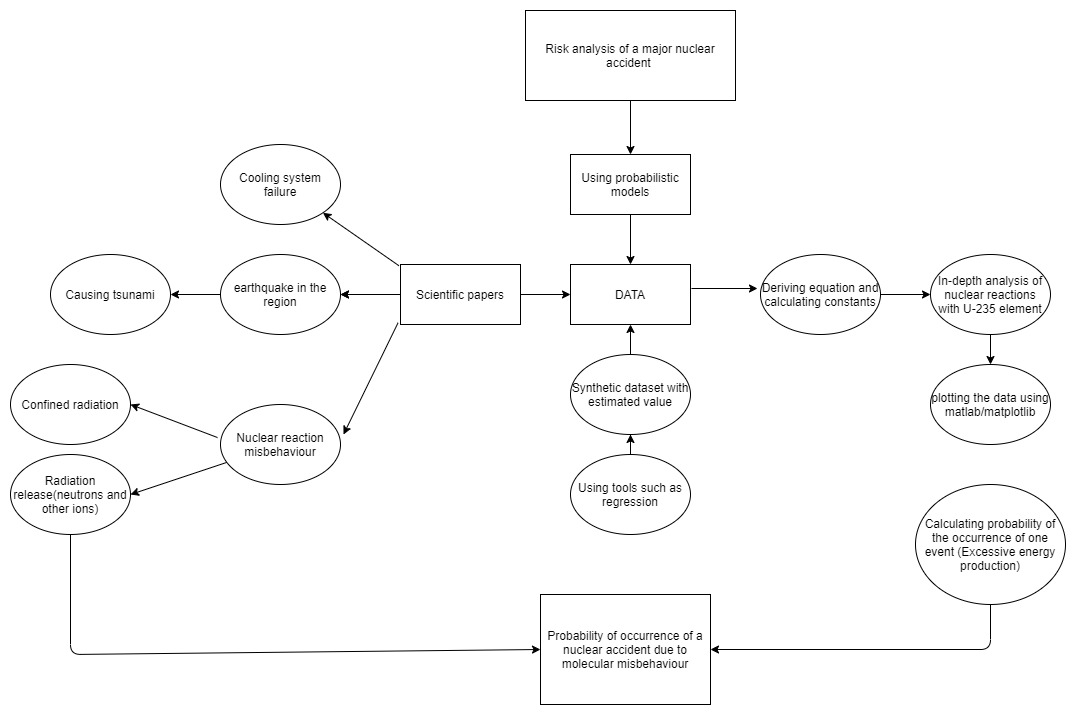
\includegraphics[scale=0.5]{Metric.jpg}
    \caption{Performance Metric}
    \label{fig:my_label}
\end{figure}


\section{Data Acquisition }
The special assignment is Data dependent. 
\begin{itemize}
    \item Datasets of nuclear power plants are confidential. So in order to calculate the probability, we have studied the existing data tables from the respective scientific papers\cite{cite9} which showed failure probability of various components and plugged those values in Joint Probability Theorem.
    \item Data regarding tsunami study was acquired from various scientific papers and websites.Graphs with discrete data values(G-R model fitting) was produced by generating random numbers in a range and plotting them. Then Curve fitting was applied to get the data required. Various algorithms for aftershock/foreshock removal (data cleaning)\cite{cite14} were used.Some data was assumed by determining the pattern of the graphs.
\end{itemize}
\section {Probabilistic Model Used}
\begin{itemize}

\item \large \textbf{Formulation}\\
The purpose of a PTHA(Probabilistic Tsunami Hazard Analysis) is to find the probability that a certain tsunami hazard metric, such as maximum wave
amplitude, is exceeded. The most basic outcome of such an analysis is typically expressed as a hazard curve,
which shows exceedance level of the hazard metric as a function of probability, with the probability often
expressed as a rate of exceedance per year.\\

Consider a PTHA includes a finite set of hypothetical tsunami-genic events e $\in$ E, with each individual event e recurring randomly in time and independently of all other events (i.e., as a Poisson process), with a known mean annual rate $\lambda(e)$(events/year). For example, E could be a set of
tsunamigenic earthquake scenarios representing all possible earthquakes affecting the site of interest, and for each earthquake event e, the mean annual rate $\lambda(e)$ might be derived based on a regional earthquake
magnitude-frequency relation: $$log[N(m)]=a-bm$$
where N(m) is the number of earthquakes greater than or equal to m and the two parameters include the activity or occurrence rate (a value) and power law magnitude exponent (b value).\\

Suppose further that for all e $\in$ E, the (spatially variable)
tsunami intensity parameter $I(x|e)$ is known at a set of locations x $\in$ X. For example, $I(x|e)$ might be taken as the peak wave height at location x due to the tsunami generated by event e. In practice, tsunami intensity measures are often derived by numerical modeling tsunami propagation for all events e $\in$ E and storing the results at a set of points x ∈ X (Pareto distribution). Under these conditions, the tsunami hazard curve at any location x describes the mean annual rate $\lambda$(events/year) at which any tsunami event occurs at location x with intensity I(x) greater than
some threshold $I_{0}$:
$$\lambda(I(x)>I_{0})=\Sigma_{e\intE}(I_{I(x|e)>I_{0}}\lambda(e))$$

Here $I_{I(x|e)>I_{0}}$ is an indicator function which takes the value 1 if $I(x|e)>I_{0}$, and zero otherwise. The above equation should be considered as a hazard curve specific to location x, which maps values of the tsunami intensity $I_{0}$ to their rate of exceedance $\lambda$.\\

The rate of exceedance is often transformed into other equivalent measures to aid its interpretation. For example, it may be converted into the probability of exceedance once or more in a given time period(with duration $\Delta T$ in years),denoted $P(I(x)>I_{0},\Delta T)$.It is computed as 
$$P(I(x)>I_{0},\Delta T)=1-e^{-\lambda(I(x)>I_{0})\Delta T}$$. The following figure shows hazard curve of Sydney offshore.\\
\begin{center}
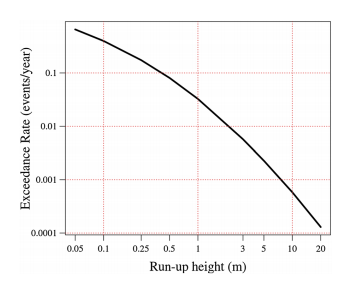
\includegraphics[]{exceedance.PNG}
\end{center}





\item \textbf{Distribution of tsunami events triggered by seismic events at a global scale:}\\
     Determining the likelihood of a disaster is a key component of any comprehensive hazard assessment. This is particularly true for tsunamis, even though most tsunami hazard assessments have in the past relied on scenario or deterministic type models. We discuss probabilistic tsunami hazard analysis (PTHA) from the standpoint of integrating computational methods with empirical analysis of past tsunami runup.
     Since tsunamis resulting from multiple seismic sources operating at different recurrence intervals can affect a given coast, the best probability model is one that is time-independent, such as a Poisson process built around an exponential distribution studied above.\\
      To describe the earthquake sizes in the target region(the term f(M)),a truncated Gutenberg–Richter relationship\cite{cite8} is adopted: \\
    $$G(M)=\frac{1-10^{-b(M-M_{min})}}{1-10^{-b(M_{max}-M_{min})}}$$ \cite{cite2}
    where Mmin and Mmax are the minimum and maximum moment magnitudes, respectively.\\
    The Gutenberg–Richter b‐value determines the ratio between large and small events; for example, a b‐value equal to 1 means that the frequency of events of magnitude M=2 is 10 times that for events of magnitude M=3\\
    \\
    For the simulation, it is convenient to convert the continuous distribution of magnitudes into a discrete set of values ($M_{min}$, …, Mi, …, $M_{max}$), assuming that they are the only possible magnitudes; such probabilities are computed as follows:\\
    \begin{center}
        P($M_{i}$)=G($M_{i}$+0.5$ \cdot \Delta M$)-G($M_{i}$ - 0.5$ \cdot \Delta M$)
    \end{center}
    
where $\Delta M$ is the discretization interval. 
For the analyses, $M_{min}$ and $M_{max}$ are set to 7.375 and 9.125, and a discretization interval of 0.25 is adopted. This means that seven central magnitude values, i.e., 7.5, 7.75, 8.0, 8.25, 8.5, 8.75, and 9.0, are considered to calculate the corresponding conditional probabilities as in the above equation. The minimum magnitude value is chosen, since small-to-moderate earthquakes rarely generate significant tsunamis, and their contributions to the tsunami hazard are negligible.\cite{cite5}\\  

Once the magnitude interval is selected and the major source area containing all possible rupture scenarios is defined, the mean annual rate of occurrence of earthquakes with magnitudes greater than or equal to 7.375 falling in that area can be calculated\cite{cite7}. Using G-R model with Poisson process for total area\cite{cite3} ,\\

Pr(Occurrence of earthquake($>$6.0 $M_{w}$) in Fukushima(100 mile radius) in one year) =$\frac{31}{15,798}$=0.001962  \cite{cite6}
\\

\newpage
\item \textbf{Application of Conditional Probability to reliability factor :}\\
\normalsize
What follows is a determination of the probability of system failure by the application of the conditional probability theorem. Figure below is the reference system. It consists of five components arranged on three "success paths. " So long as the components on at least one success path are operating, the system has not failed.\\ \\
    Probability of system failure can be written as : \\\vspace{3mm}
    \hspace{50mm}P(S)=P(S/A)P(A) + P(S/$\Bar{A}$)P($\Bar{A}$)\cite{cite9}\hspace{30mm} (1)\\
    where\\\vspace{2mm}
    \hspace{15mm}P(S)=Probability of system failure\\\vspace{2mm}
    \hspace{15mm}P(A)=Probability that component A is working (not failed)\\\vspace{2mm}
    \hspace{15mm}P(S/A)=Probability of system failure, given component A has not failed\\\vspace{2mm}
    Probability that a component is working is determined by its failure density function. For now, the derivation is beyond our scope.We will assume the following equation and move ahead. 
    $$P(\Bar{A})=\int_{0}^{t}f_{A}(t)dt \hspace{30mm} (2)$$
    $$f_{A}(t)=\beta \alpha t^{\beta-1} e^{-\alpha t^{\beta}}$$
    $\beta$=Weibull shape parameter. If $\beta$ = 1, $f_{A}(t)$ becomes the exponential failure density function.\\
    $\alpha$=Weibull scaling parameter. If $\beta$ = 1, a becomes
the failure rate , $\lambda$ \\
    and probability of no failure is \\ \vspace{1mm}
    \hspace{15mm}P($\bar{A}$)=1-P(A) \\
    where,\\ \vspace{1mm}
    \hspace{15mm}$f_{A}(t)$ = failure density function for component A\\
    P(S/A) and P(S/$\bar{A}$) can be calculated by  a stepwise application of the conditional probability theorem to the system shown in Figure.\\ \\
    \textbf{If A has not failed, the system can fail only if components B, C, and D or D or E also fail.}\\\vspace{5mm}
    \hspace{15mm}P(S/A) = P(S/A, B) P(B) + P(S/A,$\Bar{B}$) P($\Bar{B}$) \\
    Since the system will not fail if both A and B are operating then \\\vspace{5mm}
\hspace{15mm}P(S/A, B) = 0 \\ \vspace{5mm}
\hspace{15mm}$\therefore$  P(S/A) =  P(S/A,$\Bar{B}$) P($\Bar{B}$) \\
The probability of system failure given that B has failed is evaluated
as:\\ \vspace{5mm}
\hspace{15mm}P(S/A, B) = P(S/A, $\Bar{B}$, C) P(C) + P(S/A, $\Bar{B}$ , $\Bar{C}$) P( $\Bar{C}$).\hspace{30mm}(2) \\ 
The first term on the right is zero since the system cannot fail if C
has not failed. Equation (2) becomes \\ \vspace{5mm}
\hspace{15mm}P(S/A, $\Bar{B}$) =  P(S/A, $\Bar{B}$ , $\Bar{C}$) P( $\Bar{C}$)\\
The probability of system failure given that C has failed is evaluated
as:\\ \vspace{5mm}
\hspace{15mm}P(S/A,$\Bar{B}$,$\Bar{B}$) = P(S/A,$\Bar{B}$,$\Bar{B}$,D) P(D) + P(S/A,$\Bar{B}$,$\Bar{C}$,$\Bar{D}$) P($\Bar{B}$).  \\
We know if that B,C,D fails then the entire system fails. \\
\\ \vspace{2mm}
\hspace{15mm}$\therefore$ P(S/A,$\Bar{B}$,$\Bar{C}$,$\Bar{D}$)=1 \\
Similarly , calculating for E,\\ \vspace{5mm}
\hspace{15mm}P(S/A) = [1-P(E)P(D) ] [1-P(C) ] [1-P(B)]\\

P(S/$\Bar{A}$) can be calculated in the above fashion and it boils down to : \\ \vspace{5mm}
\hspace{15mm}P(S/$\Bar{A}$) - [ 1-P(E) P(D)] [l-P(C)]\\\vspace{5mm}
System failure probability is thus given by :\\
\textbf{\begin{align*}
     P(S) &= [1-P(E)P(D)] [1-P(C)][1-P(A)P(B)]\\
                  &= 0.139 \times 10^{-3} \times 0.699 \times 10^{-1} \times 0.394 \times 10^{-1}\\
                  &=0.03828 \times 10^{-5}
\end{align*}}
\begin{figure}
    \centering
    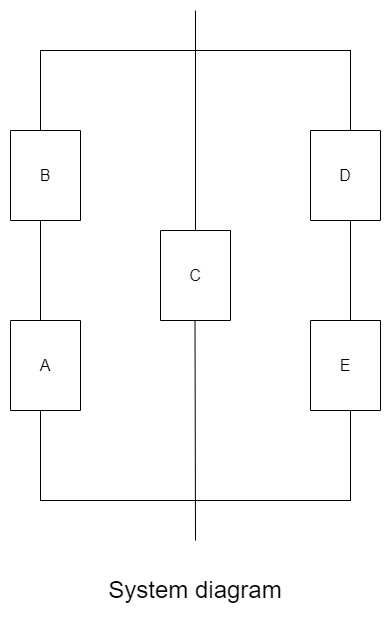
\includegraphics[scale=0.5]{System.jpg}
    \label{fig:my_label}
\end{figure}
\newpage
 \large \textbf{{\item Radiation leak :}}\\
\normalsize    There are three kinds of leak possible from a nuclear reactor, 1) Fast Neutron Leakage, 2) Thermal Neutron Leakage, 3) Gamma Ray Leakage which are equally hazardous. There are many factors that contribute to these leakage like Migration Length, Geometric Bulking, Incident Energy of Neutrons etc. 
    
    \begin{itemize}
        \item Fast Neutron Leakage :\\
            Nuclear Fission process is a Nuclear Chain Reaction. After the Fission is completed, the end products obtained are fast moving neutrons with moderator nuclei which participates further in chain nuclear reaction. But these Fast Moving Neutrons are highly energetic and must be slowed down using a moderator like water or heavy water which absorbs some amount of energy and bring the neutron in the Thermal Range.\\
            \\
            But during this process of slowing down these fast moving neutrons leak out from the reactor boundaries and escape in the form of Neutron Radiation. The probability of Fast Neutron leakage is termed as Fast Non-Leakage Probability which is calculated as,
            $$P_f = \frac{n_FL}{n_F}$$
            where $n_l$ = Number of that do not leak during the slow down process and $n$ = Total number of neutrons produced during fission.\\ 
            \\
            The Fast Non-Leakage Probability can be derived from Fermi Age Theory, which is a Stochastic Process, the probability that a neutron will remain in a core and slow down to become a thermal neutron without being lost by fast leakage, is given by the equation,
            $$P_f = e^{-\tau B^2} = \frac{1}{1 + \tau B^2}$$
            
            where, $\tau$ is Fermi Age of the neutron and B is geometric bulking factor which depends on the size and shape of reactor core and is higher for small cores and low for smaller cores. Hence it is obvious from this that fast neutron leakage is higher for smaller cores.\cite{cite10}\\
            
        \item Thermal Neutron Leakage :\\
            During Neutron Diffusion process, some thermal neutrons are leak out of the reactor core boundaries before they are absorbed by the moderator. Hence the Thermal Non-Leakage Probability is calculated as,
            $$P_t = \frac{n_TL}{n_T}$$
            where $n_TL$ = Total number of thermal neutrons leaked during diffusion process and $n_T$ = Total number of neutrons that reach thermal energy.\\
            \\
            The only parameter that influences this Non-Leakage probability is the moderator temperature. From Neutron Thermal Diffusion Theory it can be derived that a neutron will remain in the core is given by,
            $$P_t = \frac{1}{1 + L_d^2B^2}$$
            where $L_d$ is the length of diffusion which is basically the thickness of Moderator and B is the geometric bulking factor.\cite{cite11}\\
            
        \item Total Non-Leakage Probability :\\
            Fast Neutron Non-Leakage Probability ($P_f$) and Thermal Neutron Non-Leakage Probability ($P_t$) can be combined as one single term which shows us the total Non-Leakage Probability of Neutrons ($P_{NL}$) from the reactor core and can be expressed as,
            $$P_{NL} = \frac{1}{(1 + L_d^2B^2)}\cdot \frac{1}{(1 + \tau B^2)} $$
            $$P_{NL} = \frac{1}{1 + (\tau + L_d^2)B^2 + \tau L_d^2B^4}$$\\
            
            For Large reactors we can re-write $\tau + L_d^2$ as $M^2$ where M is the migration length. The term $B^4$ can be neglected for large reactors as its value is very small for large reactors and hence we can write the total Non-Leakage Probability of Neutrons as,
            $$P_{NL} = \frac{1}{1 + M^2B^2}$$
            
            Since both the factors $P_f$ and $P_t$ are dependent on the moderator temperature, the total Non-Leakage Probability is dependent on Moderator Temperature too and is sensitive to the changes in Moderator Temperature. Increase in Moderator Temperature causes an decrease in $P_{NL}$ which means more neutrons leak out of the reactor.\cite{cite13}\\
            \\
            
        \item Gamma Ray Probability :\\
            During the process of Thermalization of fast moving neutrons, neutrons may collide with moderator as well as fuel nuclei. Sometimes the reactor fuel might exhibit Resonance Behaviour between fast and thermal neutron range. During the process of Thermalization there is a chance that these intermediate energy neutrons might get Captured by the nuclei and the nuclei might go into an excited state.\\
            \\
            The probability of the neutron to escape this resonance is termed as Resonance Escape Probability which has an average value of around 0.75.\cite{cite12}\\
            \\
            Whenever the neutron is captured by the nuclei, the nuclei transmits to an excited state and comes back to normal state by emitting a Gamma Ray and a fast moving neutron. But these neutrons have a high chance of being captured at a specific Energy called Resonance Energy ($E_r$). If and incident neutron hits the nuclei with this energy then there is a high chance of nuclei undergoing Resonance.\\
            \\
            The chances of nuclei undergoing a Resonance is calculated in terms of cross-section. Cross-Section basically is the probability that when neutron and the nuclei are incident on each other. More the cross section, more is the probability of the nuclei to undergo resonance. Cross-Section is measured w.r.t to Incident energy of Neutron.\\
            \\
            Formula for Cross-Section w.r.t Incident Energy is,
            $$\sigma = \pi \Bar{\lambda}^2 \frac{\Gamma^2}{(E - E_r)^2 + (\frac{\Gamma}{2})^2}$$
            
            where $\Gamma$ = $\frac{\bar{h}}{\tau}$,$\tau$ is the half-life of the nuclei, $\Bar{\lambda}$ is the wavelength of the incident neutron and $E_r$ is the Resonance Energy. As we can see that, at Resonance Energy, the cross-section is maximized. The equation obtained above is known as the Breit-Wigner Formula which is a derived form of Cauchy-Lorentz Distribution and is derived from Quantum Theory of Radioactivity.
    \end{itemize}
\end{itemize}

\section{Derivations/Algorithms}
\begin{itemize}
    \item Obtaining the Breit-Wigner Distribution :-
    \begin{itemize}
        \item Naturally what happens is during a resonance is that there is an intermediate state $N_i^*$ which follows to a final state $N_f$ through emission of gamma rays.
        $$N_i^* \xrightarrow{} N_f + \gamma$$
        $$\Psi^{N_i^*} \xrightarrow{} \Psi^{N_f}\Psi^\gamma$$\\
        We start by assuming that the final nuclear state is given by,
        $$\Psi(\vec{x}, t) = \Psi(\vec{x})e^{iE_{i}t/h}\frac{e^\frac{-t}{2 \tau}}{\sqrt{\tau}}$$
        and this follows directly from the interpretation of probability density of excited state
        $$|\Psi^{N_f}(\vec{x},t)|^2 = |\Psi^{N_f}(\vec{x})|^2 \frac{e^{-t/\tau}}{\tau}$$
        
        Performing Fourier Transform, the above distribution is time is converted to a distribution in frequency of Fourier transform, namely,
        $$\Psi(\vec{x}, \omega) = \Psi(\vec{x})\frac{1}{\sqrt{2\pi \tau}}\int_0^\infty dt e^{i(\omega_i - \omega)t}e^\frac{-t}{2\tau}$$
        
        Performing the integral and obtaining the real valued function by replacing $\omega$ with E we get,
        
        $$|\Psi(\vec{x}, E)|^2 = |\Psi(\vec{x})|^2 \frac{\Gamma}{2\pi}\cdot\frac{1}{(E_i - E)^2 + (\frac{\Gamma}{2})^2}$$
        
        where $\Gamma = \frac{\hbar}{\tau}$. But this term obtained is the Probability Density of Energy and hence when the reaction is dominated by narrow resonances, its Cross-Section will be given by,
        $$\sigma = \pi \Bar{\lambda}^2 \frac{\Gamma^2}{(E - E_r)^2 + (\frac{\Gamma}{2})^2}$$
        
        \item Hence the controlling parameter for the Breit-Wigner Distribution for obtaining Cross-Section w.r.t to Incident Energy is $\Gamma$ which differs from element to element as it is dependent on the half-life of the respective elements ($\tau$). $\Gamma$ is responsible for the width of the curve and hence for narrow resonances, the value of $\Gamma$ is small which implies that the element is long-lived and will react to the incoming particles having definite energies near $E_r$ which is the mean of the distribution which corresponds to the maximum value of Cross-Section.
        
         
    \end{itemize}
\end{itemize}
\section{Coding and Simulation}
\begin{itemize}
    \item We already had the values of incident energy available from the ENDF database and corresponding value of $E_r$ and so we just had to calculate the value of Geometric terms because value of $\Gamma$ was known already because we already knew the half-life of 1st Meta-Stable Uranium Nuclei.
\end{itemize}
%%\subsection{Simulation Framework}
%%\justify This paragraph must include the values of all controlling parameters set in you simulations, no. of montecarlo iterations, etc.%%
\subsection{Reproduced Figures}
\begin{itemize}
\item Tools used to Reproduce these figures are Python and its corresponding libraries of Numpy, Pandas, Matplotlib and Tensorflow.
\item Reproduced Figure-1\\
\begin{figure}[htp] 
    \centering
    \subfloat{%
        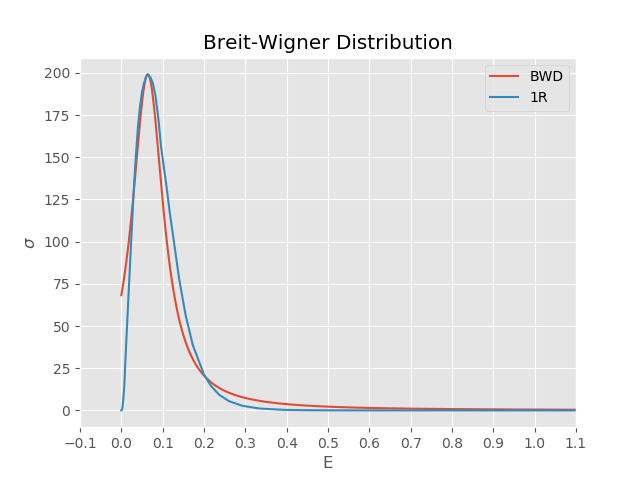
\includegraphics[width=0.5\textwidth]{bwd.png}%
        \label{fig:a}%
        }%
    \hfill%
    \subfloat{%
        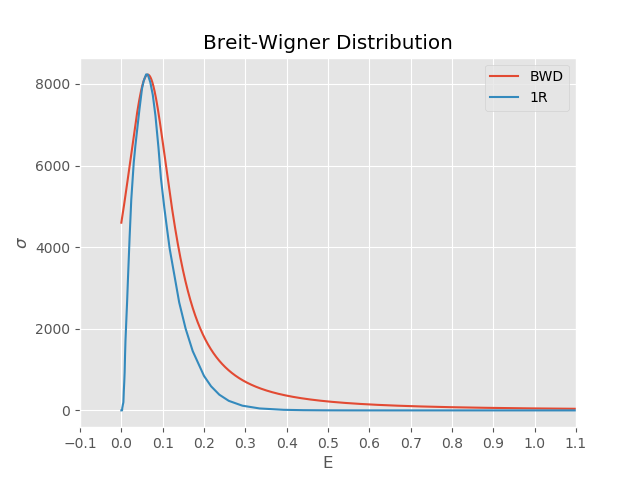
\includegraphics[width=0.5\textwidth]{bwd4.png}%
        \label{fig:b}%
        }%
\end{figure}
Curves plotted in red are the Actual Breit-Wigner Distributions plotted by feeding the values of Incident Energy in the Formula and the curves plotted in blue are the Experimental data obtained from ENDF database.\\ 
The First figure is the plot of Excited Nuclei in the First Excited state and the Second Figure is the plot of the Excited Nuclei in any given state i.e, the nuclei can be either in first or second or third and so on excited states.\\
We can see that the first figure has a maximum cross-section of 200 mb while in the second figure we can see that the maximum value of Cross-Section is about 8000 mb because it is a plot of all possible excited states or we can say that it is the addition of respective Cross-Sections of each excited state and hence it does not fall in line completely with the actual Breit-Wigner Curve while each corresponding excited state almost falls in line with actual Breit-Wigner Curve.

% Insert two figures side by side in a same row. The left figure is first figure of your base article (You can crop this). Name this as Figure 1B (Base stands for base article). And the right figure should include the corresponding reproduced figure that you have generated (along with legends). Name this as Figure 1R (R stands for reproduce figure)
% Describe the figure in detail(for e.g Figure 1B and 1R shows the plot of $P_d$ versus $P_f$) for different controlling parameters(eg. sample size) and derive the inference.
\newpage
\item Reproduced Figure-2\\
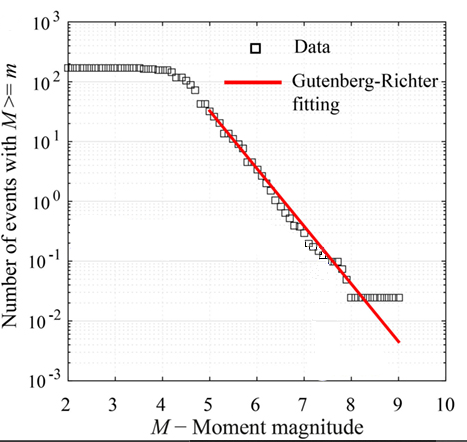
\includegraphics[scale =0.6]{gr fitting.PNG}\\
The above figure describes the plot of G-R relationship. The dataset includes only events where at least one of the magnitudes (Md, Mb or Mm) has reached the level of 2.0 and higher. Thus, we have computed the maximal magnitude of each event as the maximum of its three magnitudes (Md, Mb, and Mm).\\
The ultimate goal of this study is to predict the maximum earthquake magnitude in a given area during the next year. Thus the feature vector can include any seismic indicator, which can be calculated at the end of the current year.\\
The slope of the regression line fitting the curve of the log of the earthquake frequency versus magnitude (b value). This parameter is based on the Gutenberg-Richter inverse power law and it can be calculated using an Algorithm\cite{cite14}  from the last n events sorted in the order of their occurrence. The algorithm calls a standard Linear-Regression function, which implements the least squares linear regression method with the following input parameters:

n–the sample size (number of observations)\\
Intercept– 0 if the equation intercept is be equal to zero and 1 otherwise\\
y–n values of the dependent variable ($log_{10}(N(M))$in our case)\\
x—n values of the independent variable (M in our case)\\
\newpage
\item Reproduced Figure-3\\
 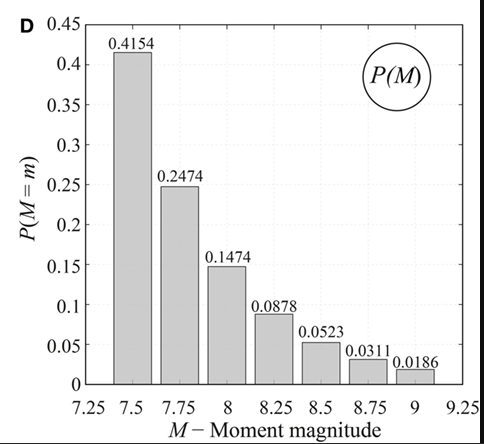
\includegraphics[scale=0.5]{P(M).PNG} 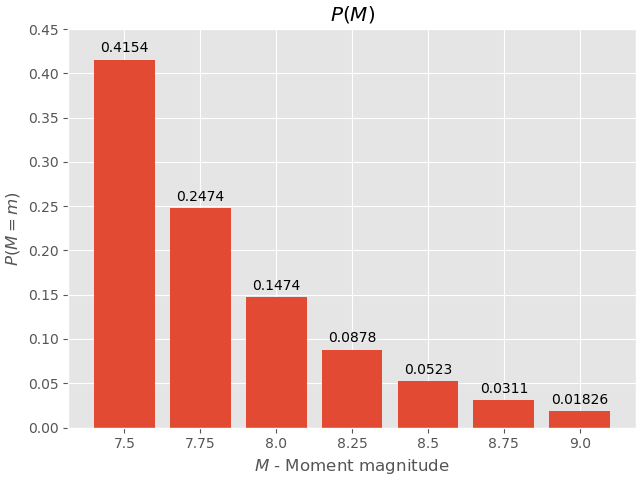
\includegraphics[scale=0.5]{plot_d.png}\\
 The above graph shows  Discrete probability mass based on the fitted Gutenberg–Richter relationship.\cite{cite3}
% Follow in the similar way as instructed above. Name the figures as Figure 2R and 2B. \\
% Describe the figure in detail and derive the inference.
\end{itemize}

% \subsection{New Work Done (Optional)}

% \subsubsection{New Analysis}

% \subsubsection{New Coding / Algorithm}

% \subsubsection{New Results}

% \subsubsection{New Inferences}
% \begin{itemize}
%     \item Describe:
% \end{itemize}

% Students are advise
% d to share the new derivations with results in correlation with the  reproduce results. Write clear inference for the new results. You are also advised to add new analysis along with the codes.


\section{Inference Analysis/ Comparison}

\begin{itemize}

\item Derive inference-1 from the work.

\item Derive inference-2 from the work.
\end{itemize}

\section{ Contribution of team members}
\subsection{Technical contribution of all team members }
\begin{table}[h]
\centering
\begin{tabular}{|l|l|l|l|}
\hline
Tasks              & Prachee       & Panth         & Dhruvil \\ \hline
Dataset collection &               &               &         \\ \hline
Code debugging and writing     &               &               &         \\ \hline
Simulating results &               &               &         \\ \hline
\end{tabular}
\end{table}
\subsection{Non-Technical contribution of all team members }
Enlist the non-technical contribution of members in the table. Redefine the tasks (e.g Task-1 as report writing etc.)
\begin{table}[h]
\centering
\begin{tabular}{|l|l|l|l|}
\hline
Tasks  & Prachee       & Panth         & Dhruvil \\ \hline
Report writing &               &               &               \\ \hline
Deriving equations &               &               &    \\ \hline
Macro/micro analysis&               &               &               \\ \hline
\end{tabular}
\end{table}


\section{Submission checklist for uploading on Google Drive}
This section provides the submission checklist for smooth and efficient submission process.  (This is for your reference and please remove this while writing your report).
\begin{itemize}

\item Soft copy of this project Report
\item Soft copy of Abstract
\item Soft copy of Concept Map 1 and 2
\item Soft copy of base article
%\item Hard copy of \textbf{turnitin report} (It should be less than 15 percent after excluding the bibliography)
\item Soft copy of analysis (hand written)
%\item Softcopy of above four documents in pan-drive/hard drive.
\item Folder of matlab codes (with proper naming)
\item Folder of reproduced results in .fig and .jpg format
%\item .pdf Scanned copy of analysis (handwritten)
\item latex (.tex) file of the project report.
\end{itemize}
%\vspace{0.5cm}

\bibliographystyle{IEEEtran}
\bibliography{ref.bib}
\end{document}
